\documentclass[border=10pt]{standalone}
\usepackage{tikz}\usepackage{amsmath}\usetikzlibrary{arrows.meta}
\begin{document}
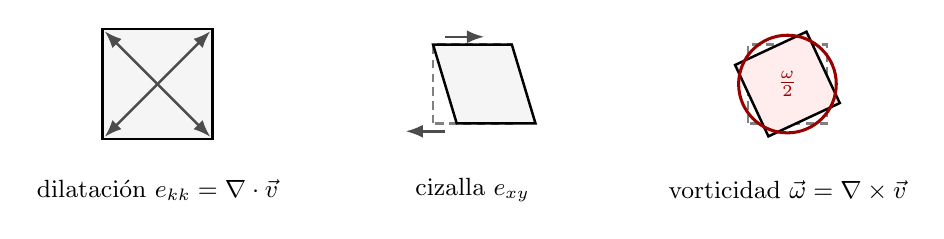
\begin{tikzpicture}[line width=0.9pt,>={Latex[length=2.2mm]}]
  % dilatacion (e_kk = div v)
  \draw[gray,densely dashed] (0,0) rectangle (1,1);
  \draw[fill=black!4] (-0.2,-0.2) rectangle (1.2,1.2);
  \foreach \a in {45,135,225,315} \draw[->,black!70] (0.5,0.5)--++(\a:0.95);
  \node at (0.5,-0.85){\small dilatación $e_{kk}=\nabla\cdot\vec v$};
  % cizalla (e_xy)
  \begin{scope}[xshift=4cm]
    \draw[gray,densely dashed] (0,0) rectangle (1,1);
    \draw[fill=black!4] (0.3,0) -- (1.3,0) -- (1.0,1) -- (0,1) -- cycle;
    \draw[->,black!70] (0.15,1.1)--++(0.5,0); \draw[->,black!70] (0.15,-0.1)--++(-0.5,0);
    \node at (0.5,-0.85){\small cizalla $e_{xy}$};
  \end{scope}
  % vorticidad (rotacion rigida)
  \begin{scope}[xshift=8cm]
    \draw[gray,densely dashed] (0,0) rectangle (1,1);
    \draw[fill=red!7,rotate around={25:(0.5,0.5)}] (0,0) rectangle (1,1);
    \draw[->,red!60!black,line width=1.1pt] (0.5,0.5) circle(0.62);
    \node[red!60!black] at (0.5,0.5){\small$\tfrac{\omega}{2}$};
    \node at (0.5,-0.85){\small vorticidad $\vec\omega=\nabla\times\vec v$};
  \end{scope}
\end{tikzpicture}
\end{document}
